\documentclass[12pt]{article}

\usepackage{sbc-template}

\usepackage{graphicx,url}

\usepackage[brazil]{babel}   	
%\usepackage[latin1]{inputenc}  
\usepackage[utf8]{inputenc}

\graphicspath{{./img/}}
% UTF-8 encoding is recommended by ShareLaTex 			

% \usepackage{natbib}
% 
% \setcitestyle{authoryear, open={((},close={))}}
     
\sloppy

\title{Sistemas Gerenciadores de Conteúdo e de Aprendizagem}

\author{Inalberth P. Santos\inst{1}, Ramon C. Gusmão\inst{1}, Ramon V. S. Bezerra\inst{1}}

\address{Instituto Federal de Educação, Ciência e Tecnologia do Maranhão\\
  Av. Getúlio Vargas, 04 -- São Luís -- MA -- Brasil
  \email{\{inalberth07, ramoncgusmao, ramonbezerra90\}@gmail.com}
}

\begin{document} 
    
\maketitle

\begin{abstract}
  The purpose of this paper is present Content and Learning Management Systems, which are organised in three basic categories: content, learning and the third one 
  based on content and learning, explaining their origins, characteristics, usage and relations among them, as well as showing their similarities 
  and differences, since even today such terms are used incorrectly, contributing to a possible wrong choice for a company or educational 
  institution to acquire such a project.
\end{abstract}
     
\begin{resumo} 
  O objetivo deste artigo é apresentar os Sistemas de Gerenciamento de Conteúdo e Aprendizagem, os quais se dividem em três categorias básicas:
  conteúdo, aprendizado e o terceiro baseado em ambos aprendizado e conteúdo, abordando suas origens, características, aplicações e por fim 
  relacioná-los, exibindo suas semelhanças e diferenças, visto que mesmo hoje o emprego destes termos ocorre de maneira incorreta, o que pode 
  resultar em uma escolha equivocada para uma empresa ou instituição de ensino ao conceber um projeto deste segmento.
\end{resumo}

\section{Introdução} \label{sec:introducao}

Segundo \cite{phillipo2012link}, os sistemas gerenciadores de conteúdo e aprendizagem são o \emph{``elo perdido''} que interliga as reformas na 
educação contemporânea com o uso criativo e efetivo da tecnologia, porém, esta por si só não é capaz de promover aprendizado. 
Logo os sistemas os quais são objeto de estudo deste trabalho se apresentam como ferramentas que possibilitam ao instrutor orientar e 
gerenciar os objetivos alcançados pelos estudantes de maneira mais eficiente. Neste trabalho serão apresentados os principais sistemas de 
gerenciamento de conteúdo e aprendizado: \emph{LMS} (gerenciador de aprendizado), \emph{CMS} (gerenciador de cursos) e \emph{LCMS} (gerenciador de conteúdos de 
aprendizagem), descrevendo suas origens, características e arquitetura, aplicações e a relação entre os mesmos, ressaltando-se o fato de que, 
apesar de haver consenso na definição de cada um, é comum o emprego incorreto dos termos.

\section{LMS (\textit{Learning Management Systems})} \label{sec:lms}

Os LMS (do inglês, \textit{Learning Management Systems}) são aplicações de \textit{software} baseadas em tecnologias Web ou não, utilizadas para 
planejar, implementar e dar suporte ao processo de aprendizagem. A TalentLMS -- plataforma de aprendizado virtual utilizada por diversas 
organizações em segmentos distintos -- faz em sua página uma breve explanação das 
palavras que compõem o termo\footnote{http://www.talentlms.com/what-is-an-lms/\#what-is-an-lms}:

\begin{itemize}
 \item \textbf{Learning,} porque você utiliza-os para entregar/receber programas de treinamento e/ou cursos educacionais, 
 \item \textbf{Management,} porque ajuda você a organizar estes cursos, isto é, criar, alterar,
 \item \textbf{System, } porque é um programa de computador.
\end{itemize}

Conforme \cite{lonn2009saving}, LMS são sistemas Web que permitem aos instrutores/alunos compartilhar materiais, enviar e receber tarefas, fazer 
apontamentos de aulas e se comunicar online. 

Desta maneira, observa-se consenso na literatura quanto à definição do termo, porém, apesar de 
conhecida a expressão, a mesma é empregada incorretamente com certa frequência, assim como confundida com outros dois tipos de gerenciadores: 
CMS e LCMS, os quais serão abordados nas seções seguintes.

\subsection{Origens}

Segundo \cite{watson2007learning}, a sigla LMS tem sua origem na expressão ILS (\textit{Integrated Learning System}), termo criado pela Jostens 
Learning, o qual faz referência a funcionalidades adicionais além dos recursos instrucionais, como gerenciamento de conteúdo e monitoramento. 
Já LMS foi utilizado pela primeira vez para descrever parte do sistema de gerenciamento do sistema de aprendizagem PLATO K-12.

\subsection{Características}

Em termos educacionais, constitui um LMS, conforme visto em \cite{bailey1992wanted}:

\begin{itemize}
 \item Objetos de Aprendizagem são organizados em lições individuais
 \item Aulas são agrupadas em um plano de ensino
 \item Um sistema de gerenciamento coleta os resultados do desempenho do estudante
 \item Aulas são disponbilizados aos alunos de acordo com o seu progresso na aprendizagem
\end{itemize}

Assim como outros \textit{softwares}, estes sistemas podem ser aplicados em um ambiente corporativo. A seguir são listadas as características 
recomendadas para a composição do mesmo, segundo a Sociedade Americana de Treinamento e Desenvolvimento:

\begin{itemize}
 \item Integração com o Sistema de Recursos Humanos.
 \item Ferramentas de administração que possibilitem o gerenciamento dos registros de usuários, perfis, conteúdos, orçamentos, agendamento para 
 aprendizes, tutores e salas de aula.
 \item Disponibilização de acesso ao conteúdo envolvendo o meio (sala de aula, \textit{online}), método (através de um orientador, 
 somente aprendiz) e aprendizes (alunos, clientes).
 \item Desenvolvimento de conteúdo (autoria, manutenção e armazenamento)
 \item Integração de conteúdo com \textit{software} de aprendizagem de terceiros
 \item Adoção dos modelos SCORM e AICC, os quais permitem importar gerenciar conteúdos seguindo padrões independentemente dos sistemas de 
 autoria utilizados para criá-los.
\end{itemize}

A imagem abaixo ilustra algumas das principais características que compõem esta categoria de sistema, conforme apresentado:

\begin{figure}[ht]
\centering
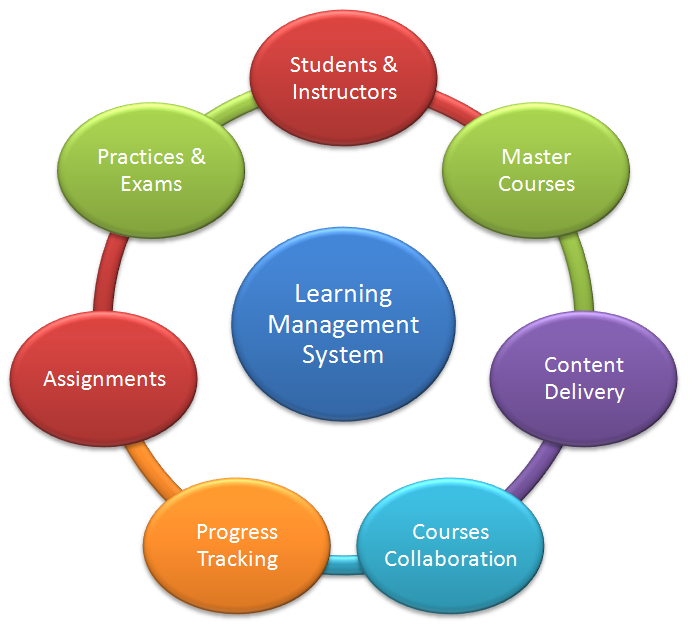
\includegraphics[width=.5\textwidth]{lmscloud.png}
\caption{Principais Funcionalidades de um LMS}
\end{figure}


Conforme \cite{watson2007learning}, o ponto principal para entender as diferenças entre LMS e outros termos relacionados à educação utilizando 
computador é compreender a natureza sistêmica dos LMS, reforçando a ideia de que este é um \textit{framework} responsável por gerenciar todos 
os aspectos do processo de aprendizagem, não se limitando, portanto, apenas à disponibilização de conteúdo, mas fazendo o gerenciamento dos 
usuários, salas de aula, cursos, análise de desempenho dos estudantes/aprendizes, acompanhando o progresso obtido, coletando e apresentando os 
dados para supervisionar o processo de aprendizagem da organização como um todo.

\subsubsection{Vantagens}

São listadas a seguir algumas das vantagens desta categoria de sistemas, apresentadas pela Mindflash\footnote{https://www.mindflash.com/lms}, 
empresa que promove treinamentos para diversas empresas:

\begin{itemize}
 \item Fácil adaptação e reuso de materiais.
 \item Mais opções para os criadores dos cursos como métodos de disponibilização, design de materiais, técnicas de avaliação.
 \item Redução de custos relacionados aos gastos com o desenvolvimento e manutenção de conteúdo por terceiros.
 \item Melhoria no desenvolvimento profissional e avaliação, permitindo a maior agregação de valor aos Recursos Humanos das companhias e ao mesmo 
 proporcionando aos empregados seu desenvolvimento individual.
\end{itemize}

\section{CMS (\textit{Content Management Systems})}

\section{LCMS (\textit{Learning Content Management System)}}

O LCMS é um sistema de aprendizagem e gerenciamento de conteúdo onde se encontra tecnologia de software relacionadas que fornece um ambiente 
multiusuário dos autores, designer instrucionais e especialista no assunto. “um LCMS gerencia o conteúdo de aprendizagem, facilita a reutilização 
de conteúdo, fornece suporte de fluxo de trabalho durante o desenvolvimento de conteúdo, e entrega de conteúdo via interfaces pré-definidas e 
camadas de apresentação” (Chapman,2001)

Os usuários podem criar o conteúdo e utilizá-lo reduzindo os esforços de desenvolvimento duplicado. Pois o conteúdo fica independente do curso 
ou disciplina e pode ser usado sempre que preciso. Outro ponto forte é que os conteúdos possuem um controle de versão e você pode se quiser 
trabalhar com uma versão anterior do mesmo conteúdo. “Os LCMS são ideais para criar estratégias de aprendizagem centrada no conteúdo, suportando 
vários métodos de criação e organização de conteúdo, alavancando conteúdo para múltiplas finalidades e conteúdo para de operações críticas .” 
(Chapman,2009)

Por que utilizar o LCMS? Porque eles utilizam cursos genéricos o que facilita na hora de criar outro curso semelhante utilizando módulos do 
anterior sem ter o trabalho de reescrever. Alguns alunos tem anseios de aprender apenas algum conteúdo especifico e não o curso volumoso e fechado, 
o LCMS está preparado para atender alunos assim pois “Para conseguir isso, os cursos de estilo antigo deve ser atomizado e dividido em pedaços de 
tamanho razoável (objetos de aprendizagem) e remontado em pacotes do tamanho certo. LCMS foram projetados para lidar em nível atômico.” (Chapman,2001). Outro fato é que um LMS foi projetado para “matrícula, frequência, listas de turmas, notas, resultados de testes, agendamento de classe, e outros requisitos administrativos das escolas e aulas ministradas por formadores de rastreamento.”(Chapman, 2001) eles não são tão bons em criar conteúdo de forma atômica ou dinâmica que para o Chapman esses pequenos conteúdos ou pedaços de aprendizagem estão no centro de um LCMS e são guardados numa base de dados central.

Para Harvi ele identifica seis características para ser um LCMS. Ele deve possuir um repositório centralizado, usar tags e ferramenta de pesquisa, 
ter recursos Compartilhado e reutilizáveis, possuir objetos de aprendizagem pequenos e reutilizáveis, controle de versão de publicação e suporte 
para os padrões da empresa.


Um exemplo pratico de um sistema LCMS é o EduLearn que é um LCMS nele se gerencia o conteúdo de aprendizagem, facilita a reutilização de conteúdo, 
fornece suporte de fluxo de trabalho durante o desenvolvimento de conteúdo, entrega de conteúdo via interfaces pré-definidas e camadas de 
apresentação. Os especialistas no assunto (PME), Designers de conteúdo e instrutores são capazes de acessar ambos banco de dados e banco de dados 
Metadados LO via seus respectivos administradores com privilégios de nível de sistema. Instrutores de usar banco de dados e banco de dados 
Metadados LO com nível de usuário privilégio ao criar os objetos do curso. Os alunos são autorizados a interagir com o conteúdo dos LCMS durante o 
seu processo de aprendizagem (Prakash,2009).

\subsection{LMS X LCMS}

“As duas ferramentas podem gerenciar e controlar conteúdo em um nível objeto de aprendizagem também.Um LMS, no entanto, pode gerenciar e 
acompanhar cursos combinados e currículo montados a partir de conteúdo on-line, eventos de sala de aula, reuniões de sala de aula virtual e uma 
variedade de outras fontes.Apesar de um LCMS não gerir aprendizagem combinada, ele faz gerenciar conteúdo em um nível inferior de granularidade do 
que um objeto de aprendizagem, que permite que as organizações para reestruturar e redirecionar o conteúdo on-line com mais facilidade.”

Além disso o LCMSs podem criar dinamicamente objetos com base em perfis de usuário e estilos de aprendizagem. Há também Tecnologias LCMS sendo 
usada em conjunto com um LMS (Chapman,2009), onde o LCMS produz e mantem salvo os LO(Objeto de Aprendizagem) e o LMS gerencia com cursos, salas, 
turmas e outras funções do LMS.

\section{Relação entre LMS, CMS e LCMS}
 
Como já mencionado, por muitas vezes os termos estudados são utilizados incorretamente

\bibliographystyle{sbc}
\bibliography{referencias}

\newpage
\appendix
\section{Linha do Tempo dos LMS}

\begin{figure}[ht]
\centering
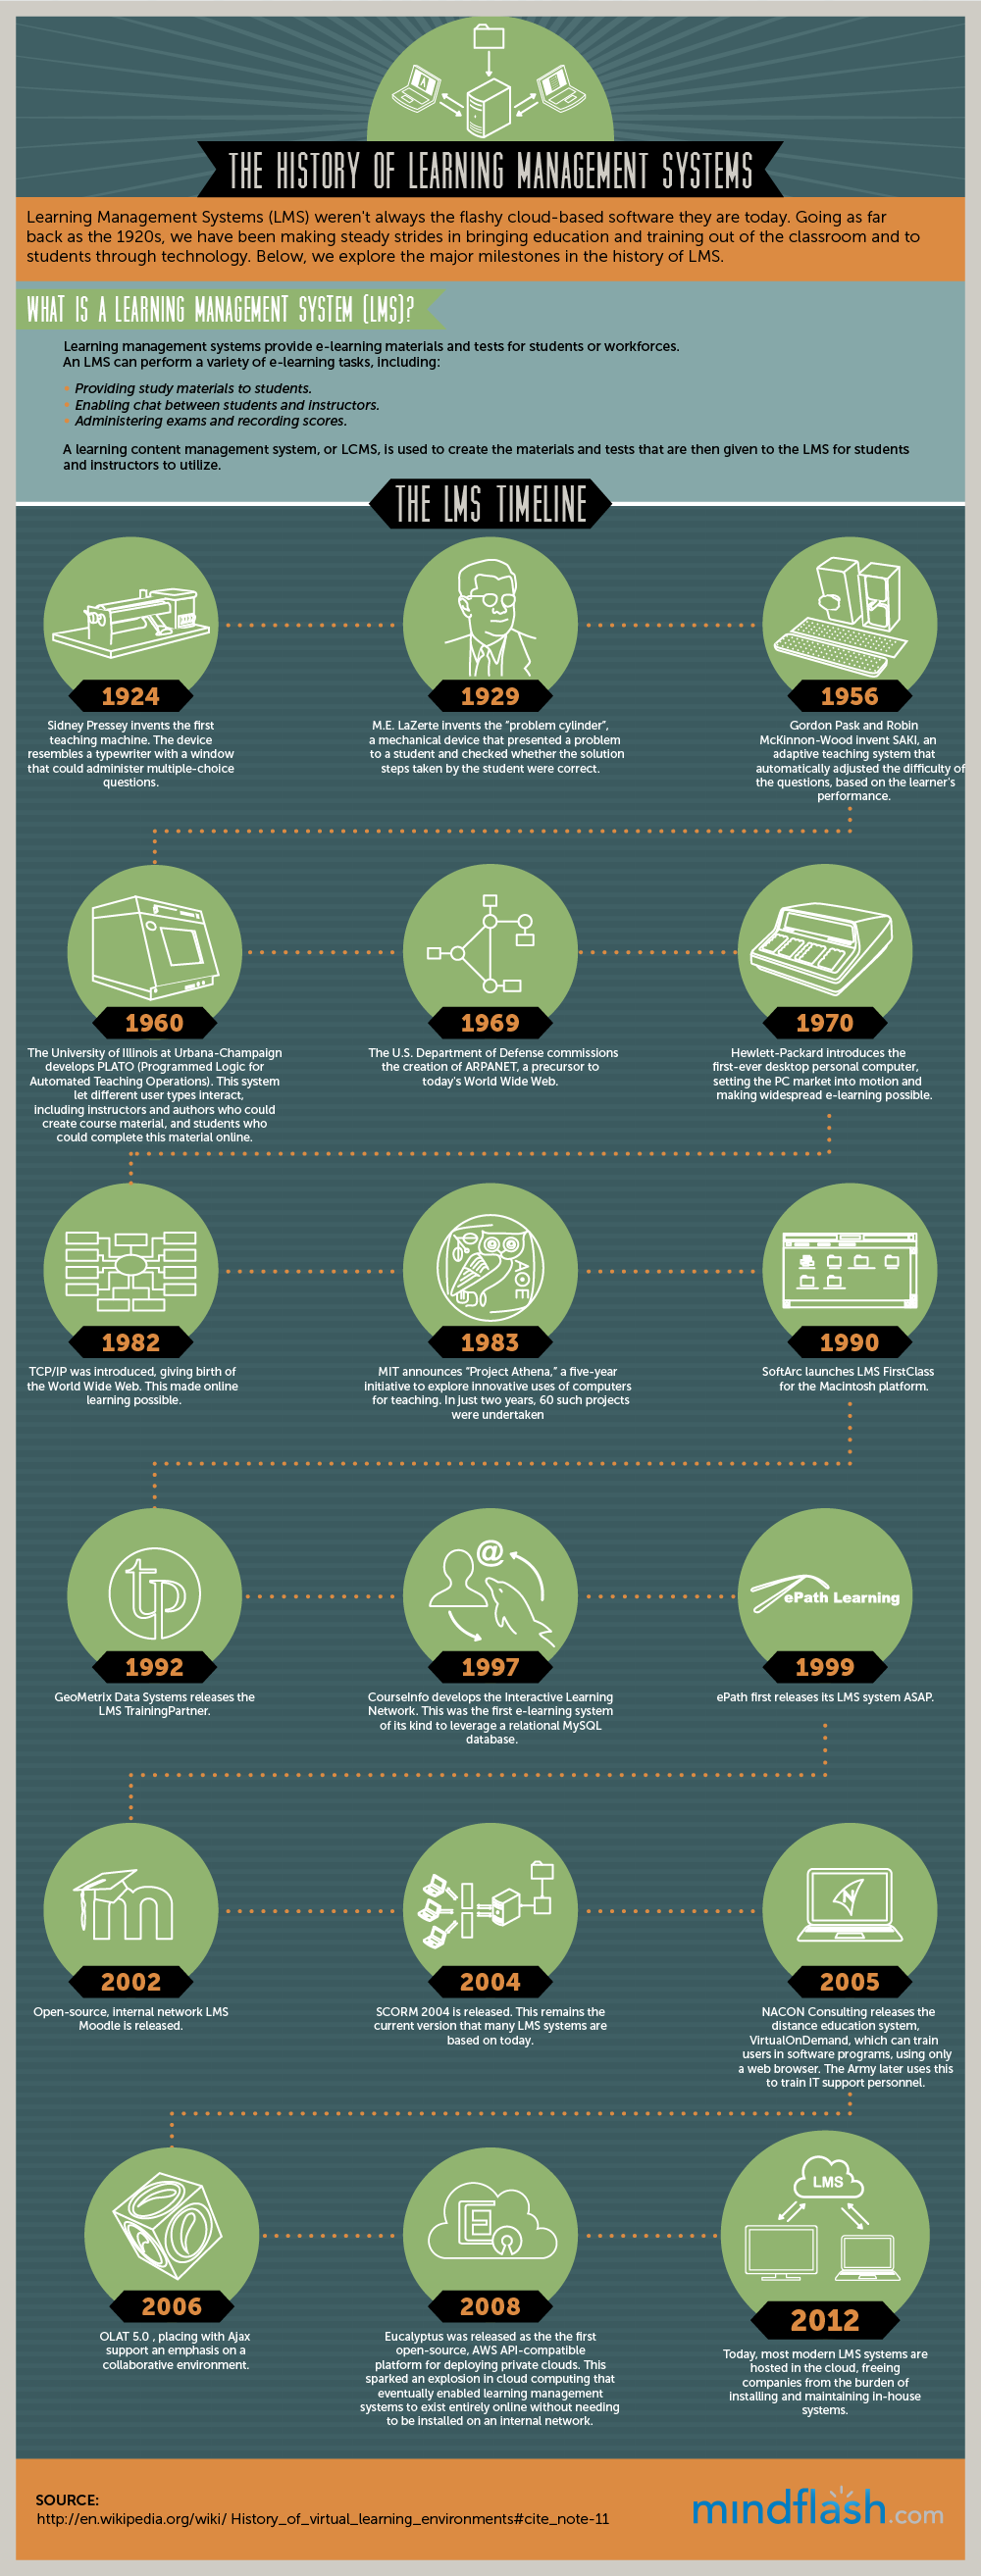
\includegraphics[width=.55\textwidth]{history-of-lms.png}
\caption{A typical figure}
\label{fig:exampleFig1}
\end{figure}

\end{document}
